\section{Design}
The concept for the GeoLog originally came from Dr. Andrew Wickert (seen in figure 
\ref{fig:andrewWickert},
which came to Reykjavík University's Mechatronics class for help developing his 
design of a low power datalogger\cite{ALog-BottleLogger}. 

\begin{figure}
\centering
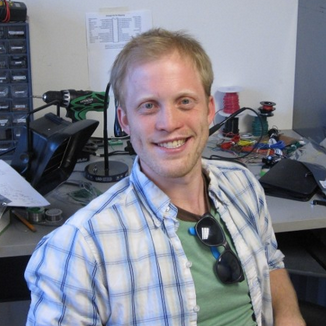
\includegraphics[width=0.6\linewidth]{graphics/andrewWickert}
\caption{Andrew Wickert\label{fig:andrewWickert}\cite{andrewWickert}}
\end{figure}

The GeoLog datalogger was designed in nine phases. Phases seven to eight were iterated
until the product was ready for deployment.
\begin{itemize}
	\item{Phase 1:} Initial brainstorming and high level design phase.
	\item{Phase 2:} Hardware selection phase, where hardware was selected and ordered.
	\item{Phase 3:} Software design phase, where the classes and interfaces were designed.
	\item{Phase 4:} Hardware hacking phase, trial and error in software writing for the
					Wixels\cite{wixel} and the GSM/GPRS module\cite{SM5100B}.
	\item{Phase 5:} Building phase, where hardware were assembled.
	\item{Phase 6:} Software integration phase, all the software integrated to one.
	\item{Phase 7:} Field testing phase, testing of the system in real life environment.
	\item{Phase 8:} Fixing phase, fixing bugs found in the field testing phase.
	\item{Phase 9:} Deployment phase, system is functional and can be deployed. 
\end{itemize}



\textit{\textcolor{red}{Assumptions stated (There are always some)}}


\subsection{Hardware}

\textit{\textcolor{red}{Description of the design; break into pieces and show how 
						they assemble.}}

\textit{\textcolor{red}{Pseudo code of important modules}}

\textit{\textcolor{red}{MDD of structure}}

\textit{\textcolor{red}{System diagram}}


\subsection{Software}
\textit{\textcolor{red}{Description of the design; break into pieces and show how 
						they assemble.}}

\textit{\textcolor{red}{Pseudo code of important modules}}

\textit{\textcolor{red}{MDD of structure}}

\textit{\textcolor{red}{System diagram}}

\subsection{Safety}
